\chapter{Implementation}

\section{Architecture Pattern \& Project Structure}
\section{Process Structure \& Inter-Process Communication}
\section{Permissions \& Android Manifest}

\section{Implementation of Concerns}
In Section (ref) we conceptualized the tasks, by decomposing the tasks into components and discussing various techniques and design decisions for implementation. In this Section, we will realize the discussion by implementing the tasks in Android. 

\subsection{Recording}
%\begin{figure}
%    \centering
%    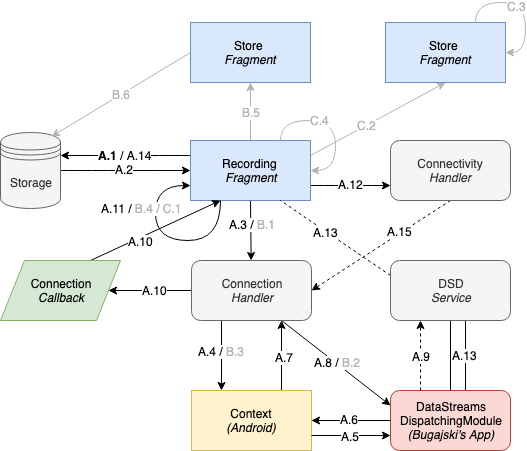
\includegraphics[scale=0.6]{images/Recording_ImpA.png}
%    \caption{Implementation of recording functionality (A)}
%    \label{fig:impl_recordingA}
%\end{figure}

%\begin{figure}
%    \centering
%    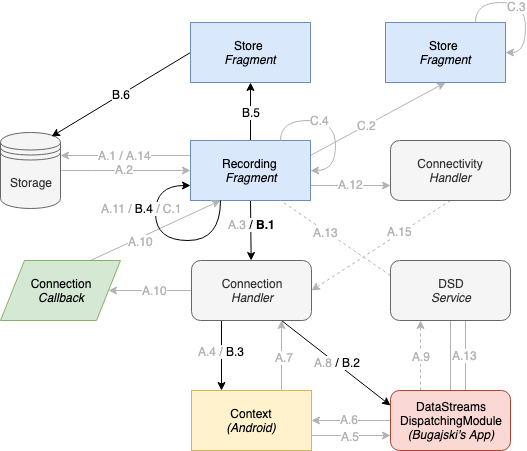
\includegraphics[scale=0.6]{images/Recording_ImpB.png}
%    \caption{Implementation of recording functionality (B)}
%    \label{fig:impl_recordingB}
%\end{figure}

%\begin{figure}
%    \centering
%    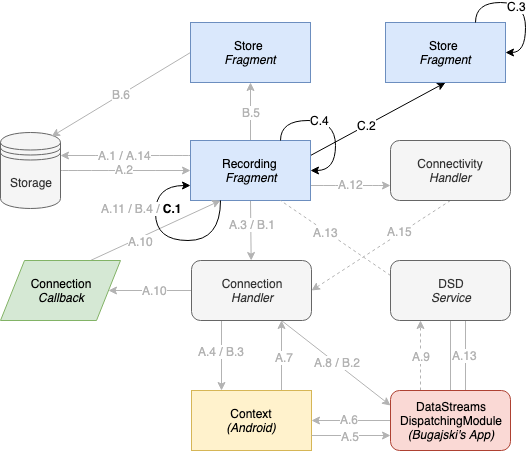
\includegraphics[scale=0.6]{images/Recording_ImpC.png}
%    \caption{Implementation of recording functionality (C)}
%    \label{fig:impl_recordingC}
%\end{figure}



\subsection{Sharing}

Sharing enables users to transmitt records across application over a media. The functionality of sharing is separated across components, to make it easier to comprehend. The actions for sharing are separated into A) exporting one or all records; and B) import a record from the device. 

Before a user can take these actions, the records from the database have to be presented. The \verb|Feed Fragment| contains a \verb|RecyclerView| which populates the records into inside the \verb|Feed Adapter| (steps: 1-4). The adapter contains all the interactions and the event handling (i.e., button event listener for exporting) for a single record. In this Subsection, we will take a look into the steps that are taken to enable the actions and imrpovements that can be made.

\begin{figure}
    \centering
    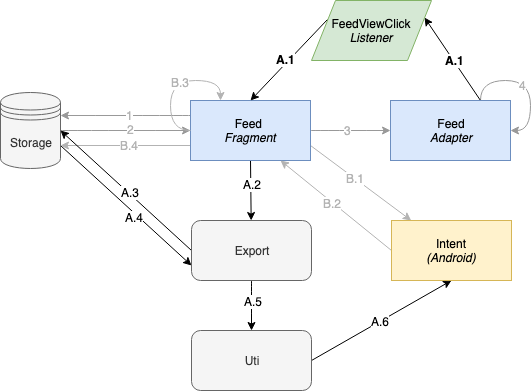
\includegraphics[scale=0.6]{images/Sharing_ImpA.png}
    \caption{Implementation of sharing functionality (A): Exporting one or all Records}
    \label{fig:impl_sharingA}
\end{figure}

\subsubsection{Action A: Exporting one or all Records}
In Figure \ref{fig:impl_sharingA}, an illustration of the steps to export one single recording is shown. However, the \verb|Feed Fragment| has an option to export all record; therefore, by disregarding the first step (A.1), the same structure applies to export all records. The steps can be narrowed down to: 

\begin{itemize}
    \item[A.1] Upon an event for exporting a selected record in \verb|Feed Adapter|, the record information is sent to the \verb|Feed Fragment| through the callback reference (\verb|onRecordAnalyticsClick|) between these components. The record information will be used to determine the corresponding samples for the record.
    \item[A.2] The \verb|Feed Fragment| delegates record information to the \verb|export| method inside of the \verb|Export| class. The class is responsible for enabling exportation. 
    \item[A.3] An operation to retrieve all samples related to the record with the use of the \verb|SampleViewModel| is done. 
    \item[A.4] The \verb|export| method retrieves all of the samples related to the record. Next, the record and the samples are encoded into an exportable JSON format (Ref: Data Format). To enable the sharing interface provided by Android, the content has to be stored on the device. Thus, the encoded data is written into a file on the device, with a filename of \verb|record_(current_date).json|, and the next component uses the reference to the file location. 
    \item[A.5] The encoded file is retrieved with the use of \verb|FileProvider| (facilitates secure sharing of files [ref]). The code for this step are
\begin{lstlisting}[language=json, caption={My Caption}, captionpos=b]
static void shareFileIntent(Activity a, File file) {

    Uri fileUri = FileProvider.getUriForFile(a.getApplicationContext(), a.getApplicationContext().getPackageName() + ".provider", file);

    Intent iShareFile = new Intent(Intent.ACTION_SEND);
    iShareFile.setType("text/*");
    iShareFile.putExtra(
        Intent.EXTRA_SUBJECT, "Share Records");
    iShareFile.putExtra(Intent.EXTRA_STREAM, fileUri);
    ...

    a.startActivity(
        Intent.createChooser(iShareFile, "Share Via"));
}

\end{lstlisting}

    \item[A.6] The user is displayed with a popup interface with several options to share the file over a media. An illustration of the layout can be found in Section Representation. 


\end{itemize}


\begin{figure}
    \centering
    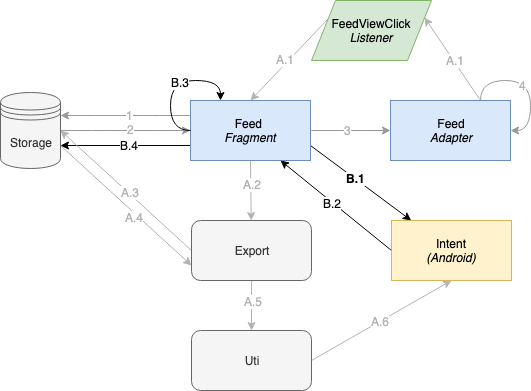
\includegraphics[scale=0.6]{images/Sharing_ImpB.png}
    \caption{Implementation of sharing functionality (B)}
    \label{fig:impl_sharingB}
\end{figure}

\subsubsection{Action B: Import a Record from the Device}
In Figure \ref{fig:impl_sharingB}, an illustration of importing a record from the device is shown. The steps can be narrowed down to:

\begin{itemize}
    \item[B.1] The user requests to view the import record interface. The interface is provided by Android, and allows the user to select particular kind of data on the device (ref). The code for this action is:
\begin{lstlisting}[language=json, caption={My Caption}, captionpos=b]
private void importRecords() {
    Intent intent = new Intent(Intent.ACTION_GET_CONTENT);
    intent.setType("*/*");
    startActivityForResult(intent, 1);
}

\end{lstlisting}
    \item[B.2] Once the user has selected the desired file, the method \verb|onActivityResult| inside of \verb|Feed Fragment| is called, and location of the selected file can be located. 
    \item[B.3] The file location is an obscured path to the file on the device; thus, parsing the path with the use of \verb|Cursor| method has to be done. After the absolute path is found, the data is decoded accordingly to the data format, and the records are sent back to \verb|Feed Fragment|.
    \item[B.4] The necessary record information and the samples are extracted from the decoded data, and are inserted into the users database. 
\end{itemize}


\subsubsection{Implementation Improvements}
The improvent for this structure is:
\begin{enumerate}
    \item In the decision of choosing a filename for the formated file (A.4), picking a filename that is easier distinguishable makes it convenient to detect on the recipients device. This could be improved by including the name of the user (e.g., \verb|record_(lastname)_(current_date).json|).
\end{enumerate}

\subsection{Modules}
Modules are standalone application, that provides data enrichment and extended functionality to the application. The modules-applications packagename is used to launch a module. The actions to enable modules in the application are A) install a module; and B) launch a module. SKRIV OM POPULATING MODULES. 

\subsubsection{Action A: Install a Module}
In Figure \ref{fig:impl_modulesB}, an illustration of installing a module shown. The steps can be narrowed down to:

\begin{figure}
    \centering
    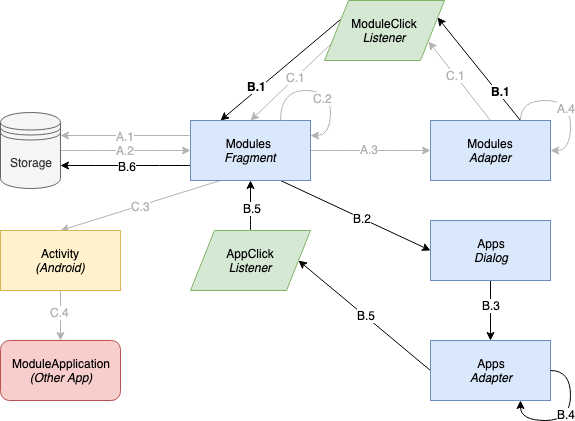
\includegraphics[scale=0.6]{images/Module_ImpB.png}
    \caption{Implementation of module functionality(A): Install a Module}
    \label{fig:impl_modulesB}
\end{figure}

\begin{itemize}
    \item[A.1] Upon an event for installing a new module in \verb|Modules Adapter|, the \verb|Feed Fragment| is notified through the callback reference (\verb|onNewModuleClick|) between these components.
    \item[A.2] The \verb|Modules Fragment| lauches a custome Android dialog, which will list all of the installed application on the device. 
    \item[A.3] The \verb|Apps Adapter| will fetch all of the application that is not a system package, already installed module, or the current application (Nidra). Next, the the adapter for the dialog will be populated with the eligible applications. 
    \item[A.4] Once the user has selected the desired module-application, an event to the \verb|Modules Fragment| through the callback reference \verb|onAppItemClick| between these components are made. The callback contains an object with the \verb|PackageInfo| for the selected module-application.
    \item[A.5] The dialog is dismissed, and the application name and packagename are extracted from the \verb|PackageInfo| for the selected module-application. 
    \item[A.6] Furthermore, the acquired information is stored in our database for modules through the DAO interface. 
\end{itemize}

\subsubsection{Action B: Launch a Module}
\begin{figure}
    \centering
    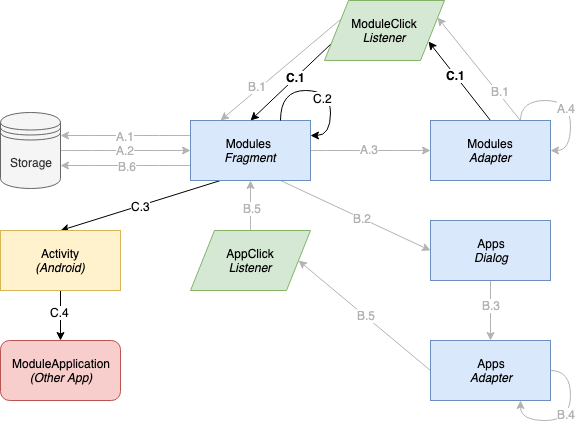
\includegraphics[scale=0.6]{images/Module_ImpC.png}
    \caption{Implementation of module functionality(B): Launch a Module}
    \label{fig:impl_modulesC}
\end{figure}

\begin{itemize}
    \item[B.1] Upon an event for launching a module in \verb|Module Adapter|, the packagename of the module is sent to the \verb|Modules Fragment| through the callback reference (\verb|onLaunchModuleClick|) between these components. The packagename  will be used to launch the module-application.
    \item[B.2] All of the records and samples on the device for the user, is bundled and formated into a JSON, and launched:
\begin{lstlisting}[language=json, caption={My Caption}, captionpos=b]
public void onLaunchModuleClick(String packageName) {
    Intent moduleApplication = context.getPackageManager().getLaunchIntentForPackage(packageName);

    if (moduleApplication == null) return;

    String data = formatAllRecordsToJSON();

    Bundle bundle = new Bundle();
    bundle.putString("data", data);

    moduleApplication.putExtras(bundle);

    startActivity(moduleApplication);
}
\end{lstlisting}

    \item[B.3] The activity uses the data provided in the \verb|Intent| that includes the packagename (the name of the module-application to determine the correct application).
    \item[B.4] The selected module is then launched, and presented to the user. The user can at anytime press the back button, to return to Nidra.  
\end{itemize}

\subsubsection{Implementation Improvements}
The improvements for the following structure are:
\begin{enumerate}
    \item During the listing of all of the installed application (A.3), only show application that are eligible module-applications. This can be achieved having a prerequisition for new modules to have a package name that starts with \verb|com.nidra.MODULE_NAME|
\end{enumerate}

%\begin{figure}
%    \centering
%    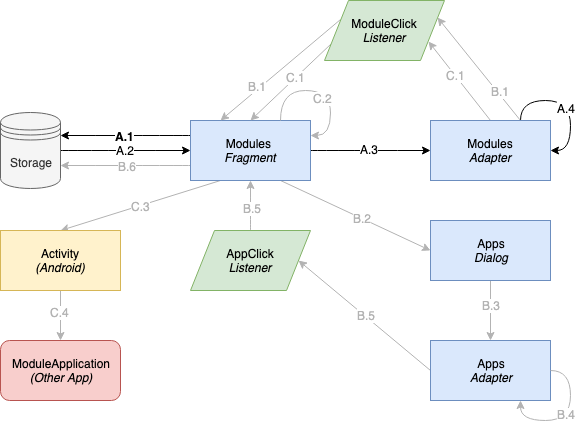
\includegraphics[scale=0.6]{images/Module_ImpA.png}
%    \caption{Implementation of module functionality(A)}
%    \label{fig:impl_modulesA}
%\end{figure}





%\subsubsection{Data Exchange Implementation}


\begin{figure}
    \centering
    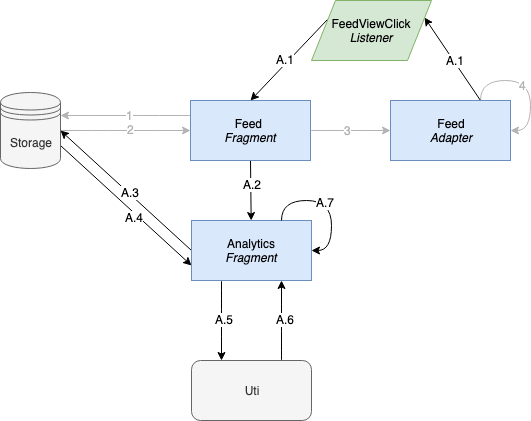
\includegraphics[scale=0.6]{images/Anal_Imp.png}
    \caption{Implementation of analytics functionality (A): Display a Graph for a Single Record}
    \label{fig:impl_analytics}
\end{figure}

\subsection{Analytics}
Analytics is the part of illustrating and analyzing the records. In Nidra, the analytics part of the implementation is limited to a time-series graph for a single record. However, there are possibilities of extending the \verb|Analytics Fragment| with other graphs based on the current structure. The current action for analytics is A) display a graph for a single record to the user. 

Similar to sharing, the records from the database have to be presented. The \verb|Feed Fragment| contains a \verb|RecyclerView| which populates the records into inside the \verb|Feed Adapter| (steps: 1-4). The adapter contains all the interactions and the event handling (i.e., button event listener for analytics) for a single record. In this Subsection, we will take a look into the steps that are taken to enable the action.

\subsubsection{Action A: Display a Graph for a Single Record}
In Figure \ref{fig:impl_analytics}, an illustration of displaying a graph shown. The steps can be narrowed down to:

\begin{itemize}
    \item[A.1] Upon an event for analytics on a selected record in \verb|Feed Adapter|, the record information is sent to the \verb|Feed Fragment| through the callback reference (\verb|onRecordAnalyticsClick|) between these components. The record information will be used to determine the corresponding samples for the record.
    \item[A.2] A new instance of the \verb|Analytics Fragment| is created, and an transition from the \verb|Feed Fragment| to the \verb|Analytics Fragment| is made. Alongside, the record information is transmitted.
    \item[A.3] An operation to retrieve all samples related to the record with the use of the \verb|SampleViewModel| is done. 
    \item[A.4] The \verb|Analytics Fragment| retrieves all of the samples related to the record. The samples has to be structured according to the graph library to display an interactive time-series graph. (GraphView (ref)).
    \item[A.5] Each sample has to be extracted from the sample-data, acccordingly to the sensor data structure.
    \item[A.6] The sample value is returned, and inserted into an array over datapoints used in the graph. 
    \item[A.7] The use is presented with a graph, which is interactable. The Y-axis has the sample value on given time (in HH:MM:SS) on the X-axis. The graph library enables interactions (e.g., zooming and scrolling) the user can do, to gain a better understanding of the recording. 
\end{itemize}



\subsection{Storage}
Storage facilites persistant data which remain available after application termination. In Nidra, there are four individual data entities (e.g., record, sample, module, and user) that are stored in a database. The access for each


\begin{figure}
    \centering
    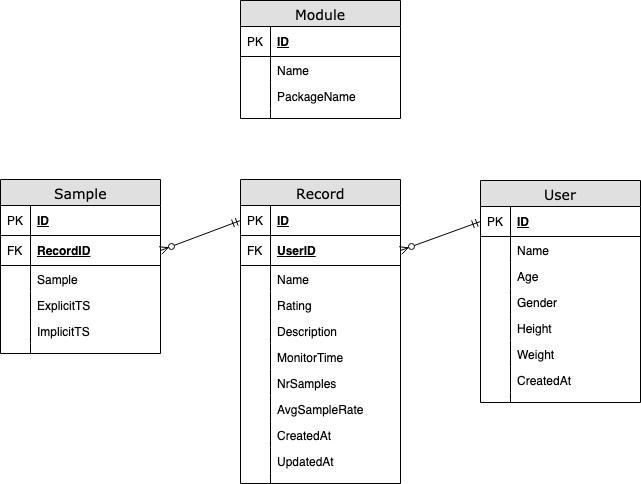
\includegraphics[scale=0.55]{images/Storage_Imp.png}
    \caption{Entity Relationship Diagram}
    \label{fig:impl_modules}
\end{figure}


\subsection{Presentation}

\begin{figure}
    \centering
    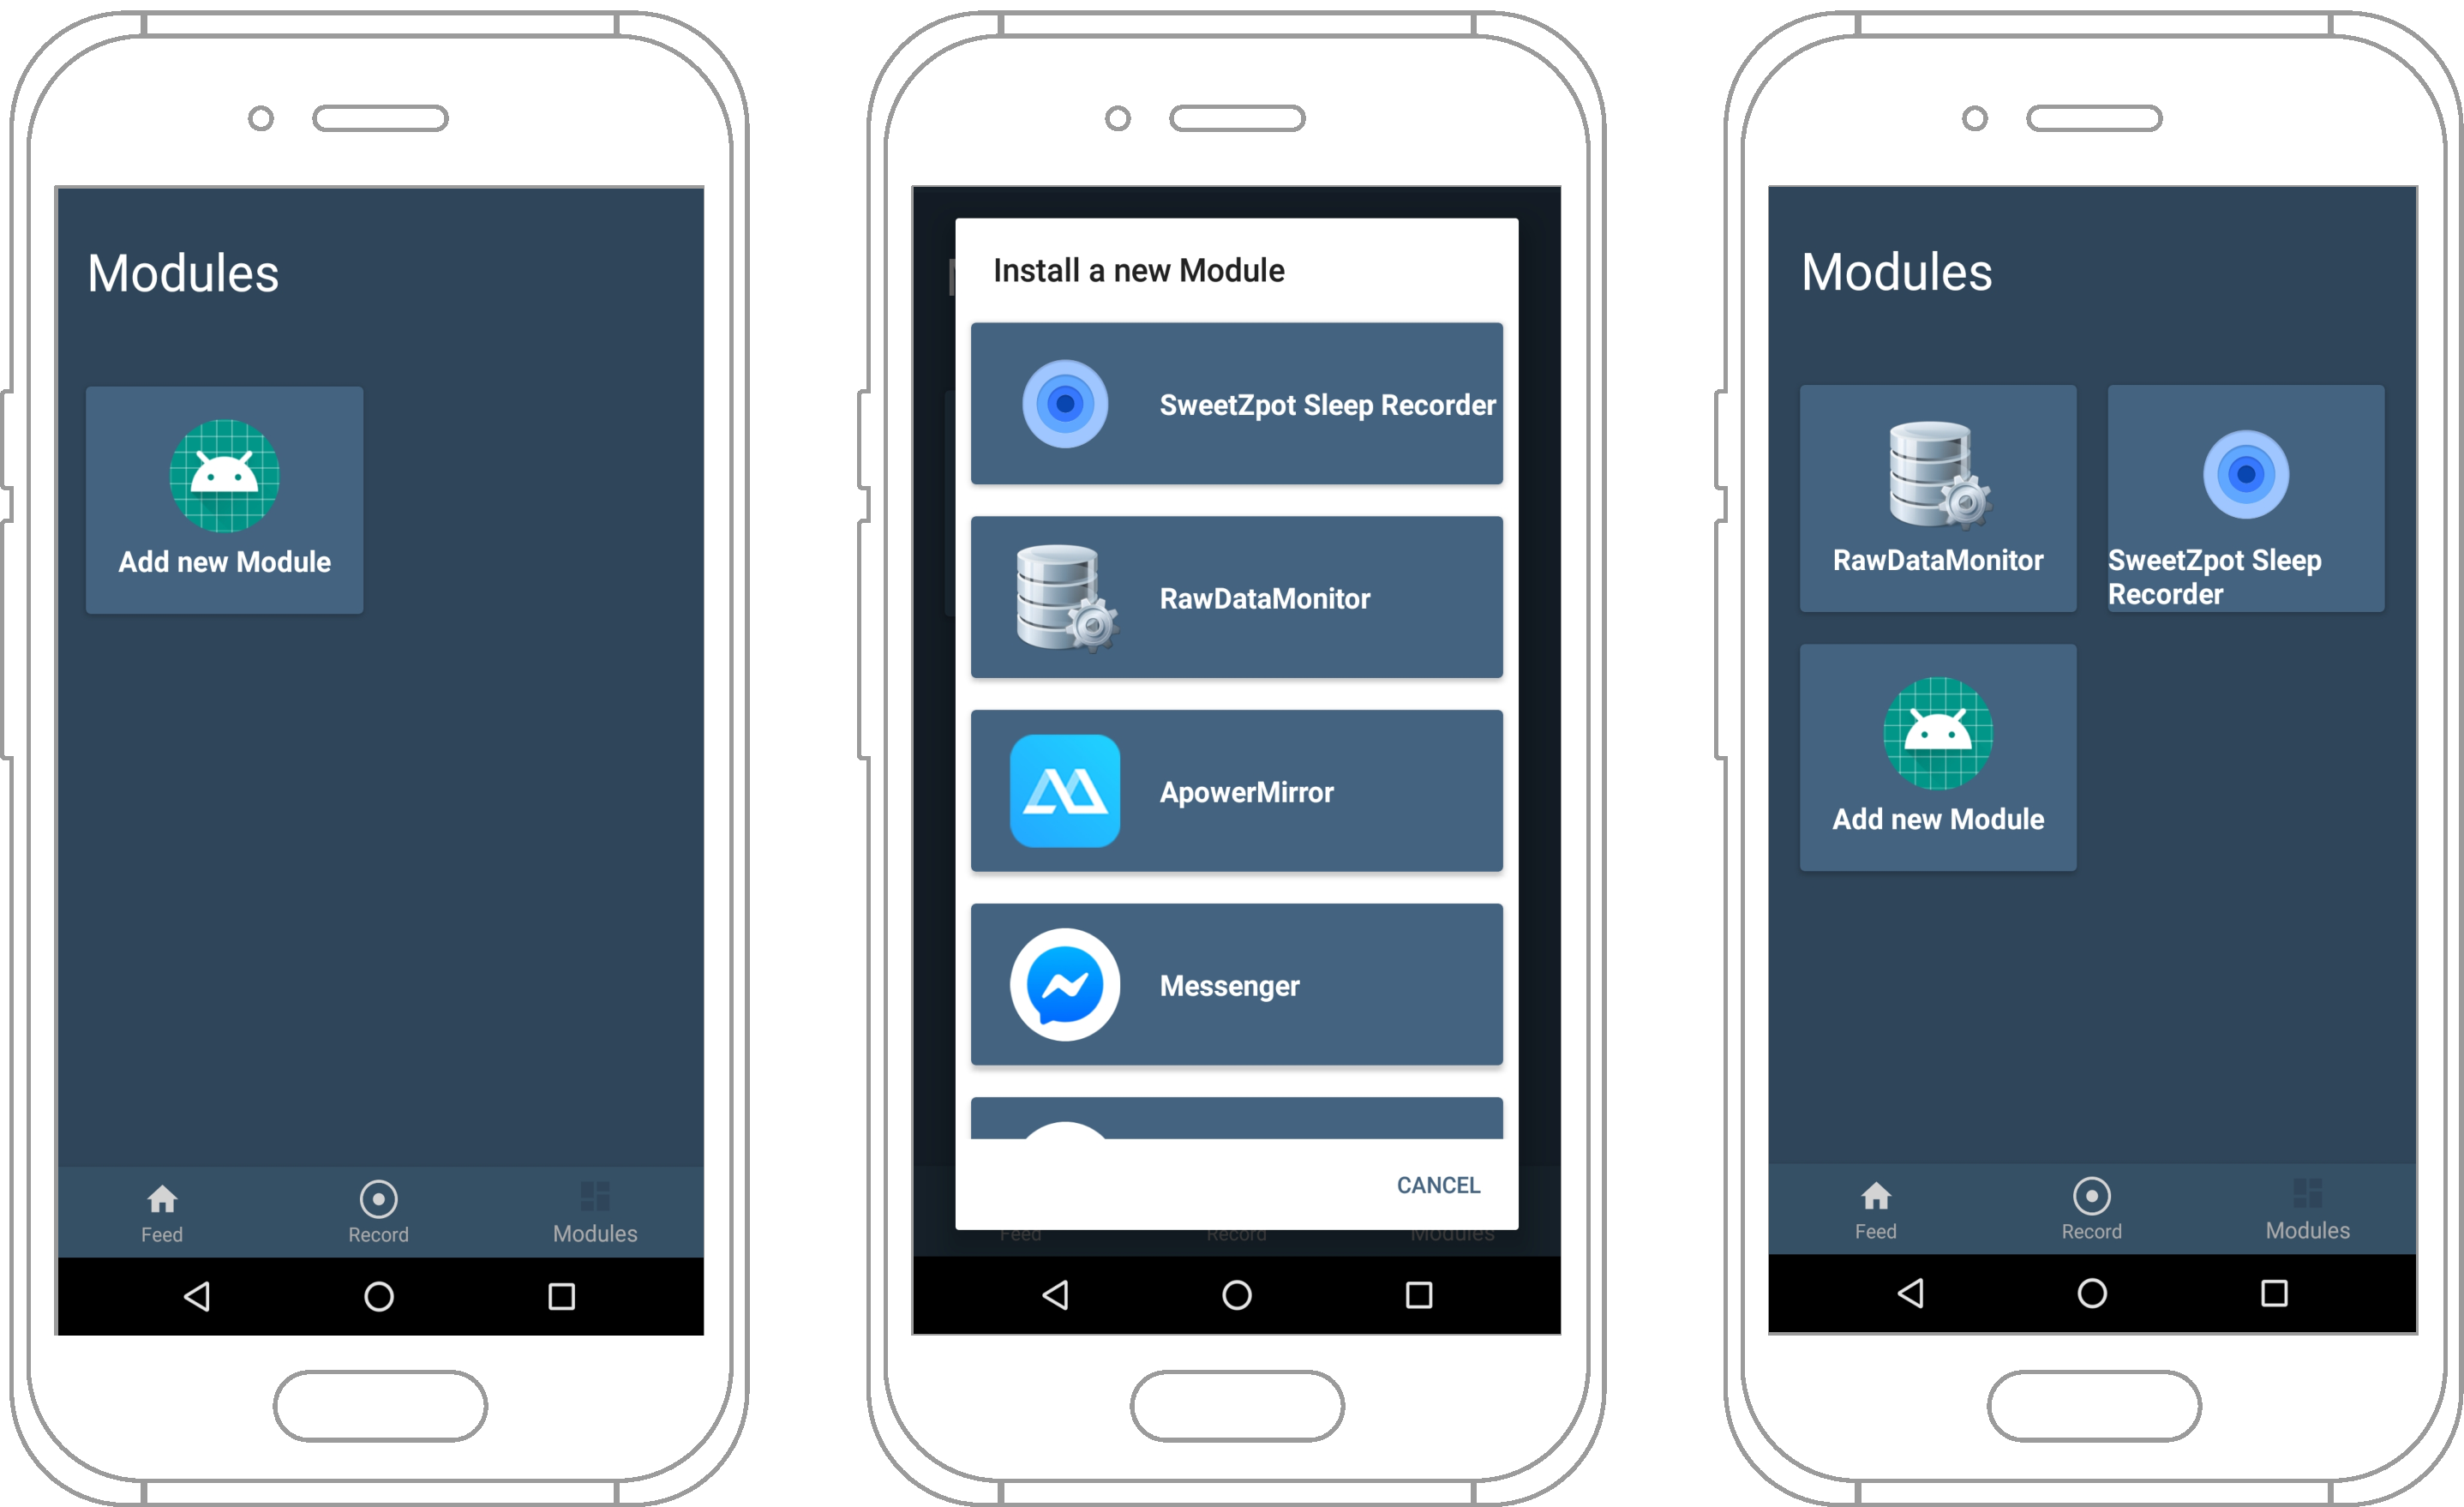
\includegraphics[scale=0.26]{images/Modules_img.pdf}
    \caption{Entity Relationship Diagram}
    \label{fig:impl_modules}
\end{figure}